\section{Estudio experimental de efecto Kerr}
\subsection{Efecto Kerr magneto-\'optico}
\frame{
	\frametitle{Tipos de efecto Kerr}
    \begin{figure}[!hbt]
    	\centering
    	\subfigure[polar]{
    		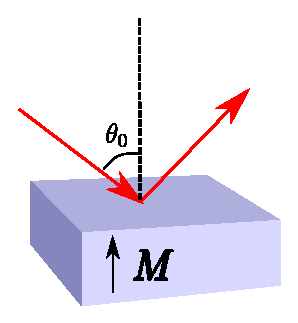
\epsfig{file=figKerr/pol/pol.eps, width=2.0cm,height=2.0cm}
    		\label{Kerr:fig:pol}
    	}
    	\subfigure[longitudinal]{
    		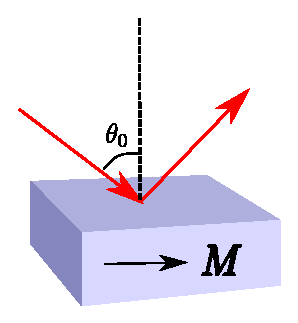
\epsfig{file=figKerr/pol/long.eps, width=2.0cm,height=2.0cm}
    		\label{Kerr:fig:long}
    	}
    	\subfigure[transversal]{
    		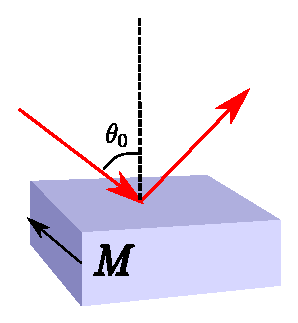
\epsfig{file=figKerr/pol/trans.eps, width=2.0cm,height=2.0cm}
    		\label{Kerr:fig:trans}
    	}
    	\caption[Configuraciones de Efecto Kerr magneto-\'optico.]{Diferentes configuraciones del efecto Kerr magneto-\'optico}
    	\label{Kerr:fig:Conf}
    \end{figure}
}